% !TeX program = lualatex -synctex=1 -interaction=nonstopmode --shell-escape %.tex

\documentclass[_Banking_p3.tex]{subfiles}
\begin{document}

\setbeamercovered{invisible}

\subsection{Нормативные документы}
\begin{frame}[allowframebreaks]{Нормативные документы}
  \begin{thebibliography}{10}
  
  \beamertemplatearticlebibitems

    \bibitem{bb2}
Федеральный закон «О драгоценных металлах и драгоценных камнях» от 26.03.1998 № 41-ФЗ (в ред. от 21.11.2011 № 327-ФЗ).

    \bibitem{bb4}
Постановление Правительства РФ от 12.12.2007 N 867 (ред. от 14.02.2009) "О выдаче кредитным организациям генеральных лицензий на экспорт аффинированных золота и серебра в виде слитков"


\pagebreak

    \bibitem{bb4}
"Кодекс Российской Федерации об административных правонарушениях" от 30.12.2001 N 195-ФЗ (ред. от 29.07.2017) (с изм. и доп., вступ. в силу с 10.08.2017). Ст.~19.14. Нарушение правил извлечения, производства, использования, обращения, получения, учета и хранения драгоценных металлов, жемчуга, драгоценных камней или изделий, их содержащих



    \bibitem{bb4}
"Уголовный кодекс Российской Федерации" от 13.06.1996 N 63-ФЗ (ред. от 29.07.2017). Ст.~191. Незаконный оборот драгоценных металлов, природных драгоценных камней или жемчуга

\pagebreak

    \bibitem{bb4}
Указ Президента РФ от 15.11.1999 N 1524 (ред. от 26.05.2008) "Об утверждении Положения об Алмазном фонде Российской Федерации"


    \bibitem{bb4}
Постановление Правительства РФ от 27.02.2003 N 127 (ред. от 17.12.2016) "Об утверждении Положения о Государственном фонде драгоценных металлов и драгоценных камней Российской Федерации"

\pagebreak

    \bibitem{bb4}
Постановление Правительства РФ от 15.02.2016 N 102 "О порядке отнесения самородков драгоценных металлов и драгоценных камней к категории уникальных" (вместе с "Правилами отнесения самородков драгоценных металлов и драгоценных камней к категории уникальных")

\pagebreak
    \bibitem{bb4}
Постановление Правительства РФ от 26.03.2001 N 233 (ред. от 08.05.2002) "Об утверждении Правил реализации на внутреннем рынке алмазов специальных размеров массой 10,8 карата и более"

  \end{thebibliography}
\end{frame}

\subsection{Определения}
\begin{frame} [ allowframebreaks]{Драгоценные металлы и камни}{Основные понятия, маркировка и оценка}
\begin{block}{ Драгоценные металлы}
\quad
- золото, серебро, платина и металлы платиновой группы (палладий, иридий, родий, рутений и осмий).
\end{block}
\pagebreak

\begin{block}{Добыча драгоценных металлов }
\quad
- извлечение драгоценных металлов из коренных (рудных), россыпных и техногенных месторождений с получением концентратов и других полуфабрикатов, содержащих драгоценные металлы.
\end{block}
\pagebreak

\begin{block}{Производство драгоценных металлов }
\quad
- извлечение драгоценных металлов из добытых комплексных руд, концентратов и других полуфабрикатов, содержащих драгоценные металлы, а также из лома и отходов, содержащих драгоценные металлы.
\end{block}
\pagebreak

\begin{block}{Аффинаж драгоценных металлов}
\quad
- процесс очистки извлеченных драгоценных металлов от примесей и сопутствующих компонентов, доведение очистки лигатуры (массы в слитке) драгоценных металлов от примесей до качества, соответствующего государственным стандартам и техническим условиям, действующим на территории Российской Федерации, или международным стандартам.
\end{block}
\pagebreak

\begin{block}{Драгоценные камни}
\quad
- минерального происхождения: природные алмазы, изумруды, рубины, сапфиры и александриты;

\quad
– органического происхождения: природный жемчуг в естественном (сырье) и обработанном виде, уникальные янтарные образования. 
\end{block}
Порядок приравнивания янтарных образований к драгоценным камням установлен Правительством РФ.

\begin{block}{Карат, англ. carat}
\quad
- внесистемная единица измерения массы, равная 200 мг (0,2 грамма). Русское обозначение: кар; международное: ct.
\end{block}
\end{frame}

\begin{frame}{Алмазы и бриллианты}{Алмаз - кристалл химически чистого углерода.\\  Бриллиант – обработанный алмаз.}
\begin{figure}	
	\centering
	\begin{subfigure}[t]{4.3cm}
		\centering
		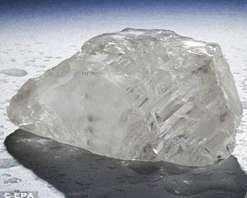
\includegraphics[scale=0.85]{img/cullinan_raw.png}
		\caption{Алмаз}\label{fig:a_cullinan_raw}
	\end{subfigure}
	\quad
	\begin{subfigure}[t]{4.3cm}
		\centering
		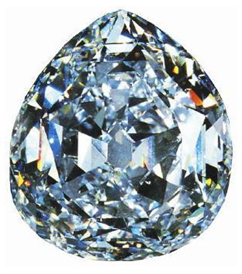
\includegraphics[scale=0.6]{img/uar_star.png}
	\caption{Бриллиант, 530.20 кар}\label{fig:b_cullinan}	
	\end{subfigure}
	\caption{Куллинан, также известен как\\ ``Звезда Южной Африки'', \\ размеры: $58.9 \times  45.4 \times  27.7$ мм, 76 граней.}\label{fig:diamonds1}
\end{figure}
\end{frame}

\begin{frame}{Известные бриллианты}
\begin{figure}	
	\centering
	\begin{subfigure}[t]{4.3cm}
		\centering
		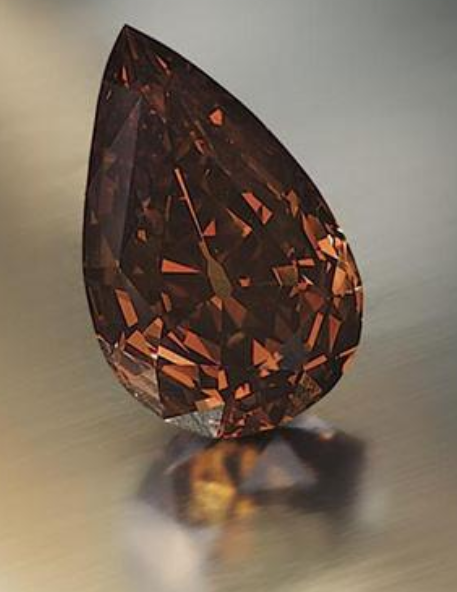
\includegraphics[scale=0.28]{img/Golden_Maharaja.png}
	\caption{Золотой Махараджа, 65.57 кар}\label{fig:Golden_Maharaja}	
	\end{subfigure}
	\quad
	\begin{subfigure}[t]{4.3cm}
		\centering
		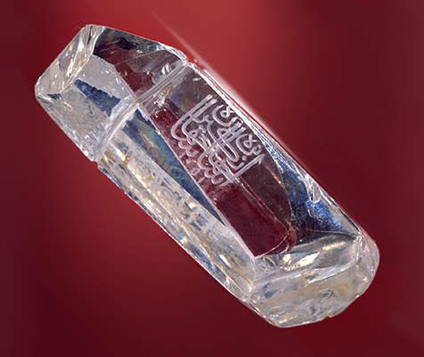
\includegraphics[scale=0.45]{img/shah.png}
		\caption{Шах, 88 кар}\label{fig:shah}
	\end{subfigure}
	\caption{Золотой Махараджа, англ. Golden Maharaja;\\ Шах, англ. Akbar Shah}\label{fig:diamonds2}
\end{figure}
\end{frame}

\begin{frame}{Известные бриллианты}
\begin{figure}	
	\centering
	\begin{subfigure}[t]{4.3cm}
		\centering
		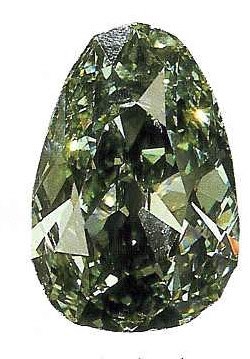
\includegraphics[scale=0.55]{img/drezden1.png}
	\caption{Дрезденский зеленый бриллиант, 40.70 кар}\label{fig:drezden1}	
	\end{subfigure}
	\quad
	\begin{subfigure}[t]{4.3cm}
		\centering
		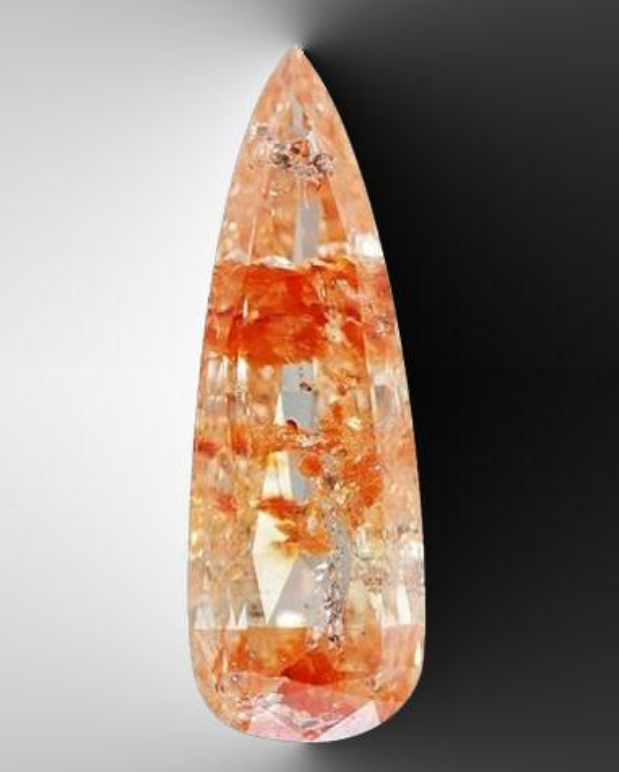
\includegraphics[scale=0.25]{img/koi_diamond.png}
		\caption{Кои Алмазный, 32 кар}\label{fig:koi_diamond}
	\end{subfigure}
	\caption{}\label{fig:diamonds3}
\end{figure}
\end{frame}


\begin{frame}{Изумруд}{– минерал бериллия с включением\\ в кристаллическую решетку ионов хрома}
\begin{figure}	
	\centering
	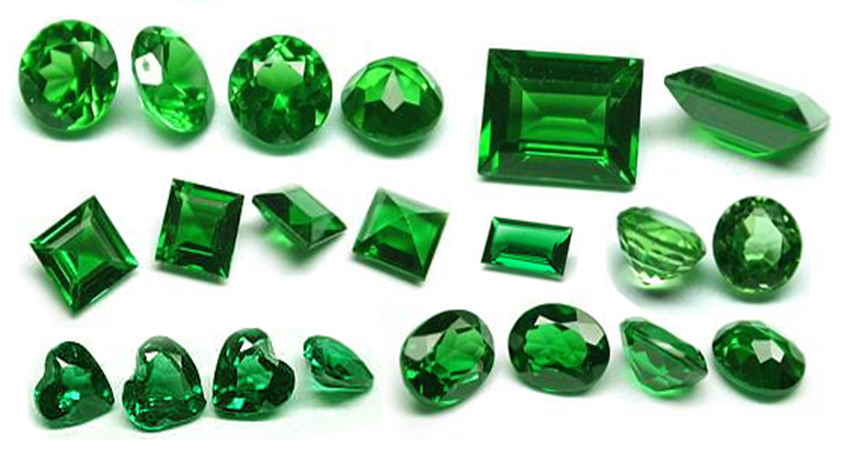
\includegraphics[scale=0.55]{img/emeralds.png}
	\caption{Изумруды}\label{fig:emeralds}
\end{figure}
\end{frame}

\begin{frame}{Александрит }{– хризоберилл (сложный оксид бериллия и алюминия)}
\begin{figure}	
	\centering
	\begin{subfigure}[t]{4.3cm}
		\centering
		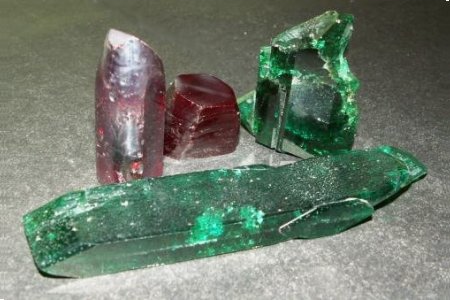
\includegraphics[scale=0.45]{img/alexandrite1.png}
	\caption{}\label{fig:alexandrite1}	
	\end{subfigure}
	\quad
	\begin{subfigure}[t]{4.3cm}
		\centering
		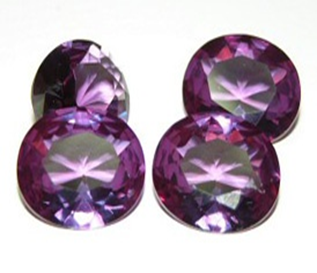
\includegraphics[scale=0.55]{img/alexandrite2.png}
		\caption{}\label{fig:alexandrite2}
	\end{subfigure}
	\caption{Александриты}\label{fig:alexandrites}
\end{figure}
\end{frame}
\begin{frame}{Сапфир }{– разновидность корунда (кремния – $SiO_2$) с включением\\ в кристаллическую решетку ионов железа и титана}
\begin{figure}	
	\centering
	\begin{subfigure}[t]{4.3cm}
		\centering
		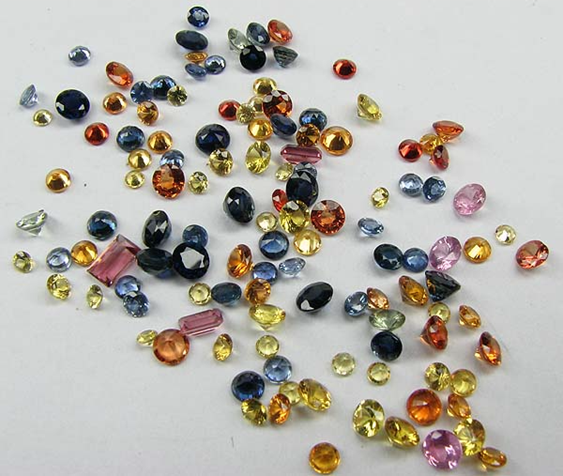
\includegraphics[scale=0.45]{img/sapphire1.png}
	\caption{}\label{fig:sapphire1}	
	\end{subfigure}
	\quad
	\begin{subfigure}[t]{4.3cm}
		\centering
		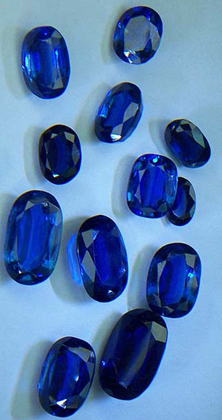
\includegraphics[scale=0.5]{img/sapphire2.png}
		\caption{}\label{fig:sapphire2}
	\end{subfigure}
	\caption{Сапфиры}\label{fig:sapphires}
\end{figure}
\end{frame}

\begin{frame}{Рубин }{– разновидность корунда с включением\\ в кристаллическую решетку ионов хрома}
\begin{figure}	
	\centering
	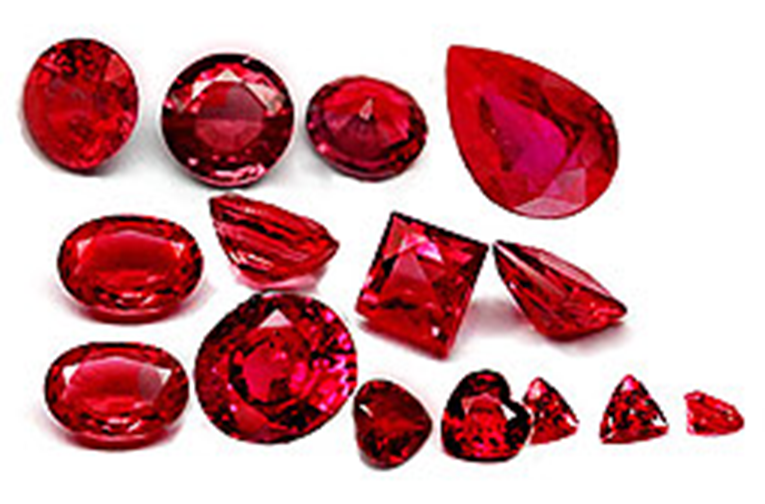
\includegraphics[scale=0.5]{img/ruby.png}
	\caption{Рубины}\label{fig:ruby}
\end{figure}
\end{frame}

\begin{frame}{Янтарь }{– ископаемая смола деревьев хвойных пород палеогенного периода}
\begin{figure}	
	\centering
	\begin{subfigure}[t]{4.3cm}
		\centering
		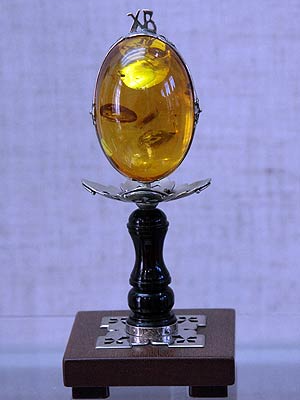
\includegraphics[scale=0.45]{img/amber1.png}
	\caption{}\label{fig:amber1}	
	\end{subfigure}
	\quad
	\begin{subfigure}[t]{4.3cm}
		\centering
		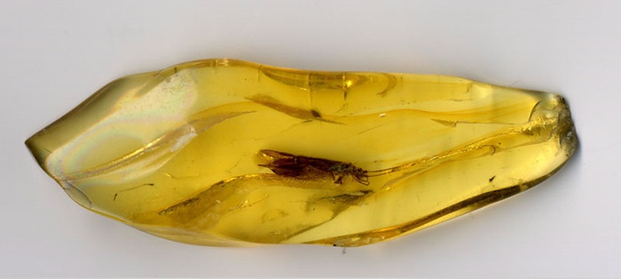
\includegraphics[scale=0.35]{img/amber2.png}
		\caption{}\label{fig:amber2}
	\end{subfigure}
	\caption{Янтарь}\label{fig:amber}
\end{figure}
\end{frame}
\begin{frame}{Жемчуг }{– секрет желез особого моллюска – жемчужницы,\\ её разновидностей – морской и речной}
\begin{figure}	
	\centering
	\begin{subfigure}[t]{4.3cm}
		\centering
		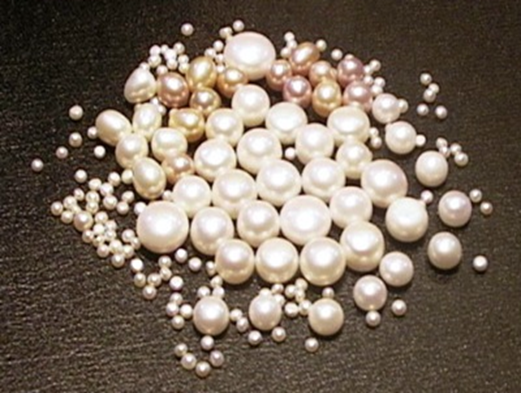
\includegraphics[scale=0.45]{img/pearls.png}
	\caption{}\label{fig:pearls}	
	\end{subfigure}
	\quad
	\begin{subfigure}[t]{4.3cm}
		\centering
		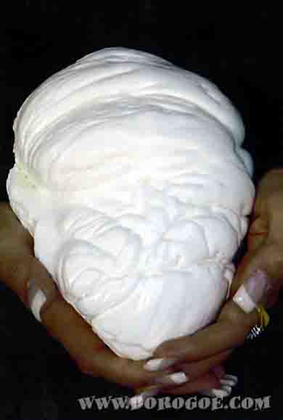
\includegraphics[scale=0.4]{img/pearl_big.png}
		\caption{}\label{fig:pearl_big}
	\end{subfigure}
	\caption{Жемчуг}\label{fig:pearls1}
\end{figure}
\end{frame}

\begin{frame}{Драгоценные металлы}{Стандарты выпуска }
- слитки стандартного веса для Ag, Au, Pt и Pdж; 

- мерные слитки (весом от 1 кг и менее для Ag, Au, Pt и Pd и остальных драгоценных металлов), 

- прокат (полос, пластин, проволоки), 

- гранулы, 

- порошок, 

- монеты и медали.
\end{frame}
\begin{frame}[allowframebreaks]{Проба металла}
\begin{block}{Проба }
\quad
– процентное содержание драгоценного металла в сплаве, из которого изготовлены слитки, прокат или порошок (количество долей чистого металла в общей массе сплава). Она обозначается двумя, тремя или четырьмя цифрами после запятой. 
\end{block}

\pagebreak
Например, проба «Четыре девятки» (0,9999) означает, что в лигатуре слитка наличие примесей составляет не более 1 части на 1000 частей сплава (1 грамм на 1 килограмм сплава). Проба может быть обозначена и в виде процента, например 99,99\%.
\end{frame}

\begin{frame}[ allowframebreaks]{Лигатура}
\begin{block}{Лигатура}
\quad
— сплав из двух и более компонентов, предназначенный для введения в жидкий металл тугоплавких элементов.
\end{block}

\pagebreak
В ювелирном деле лигатура добавляется к драгоценному металлу для доведения ювелирного сплава до определённой пробы, для изменения цвета сплава, а также для придания ему различных полезных свойств:

    - Увеличение твёрдости, износоустойчивости металла. 
    
    - Улучшение ковкости, литейных свойств, повышение/понижение температуры плавления сплава для удобства обработки изделий ювелиром.

\pagebreak
Для золота лигатура как правило состоит из серебра и меди, реже добавляются платина, палладий, никель и цинк.
\end{frame}

\begin{frame}
\begin{table}
	\center
	\caption{ГОСТы, установленные на слитки драгоценных металлов}
	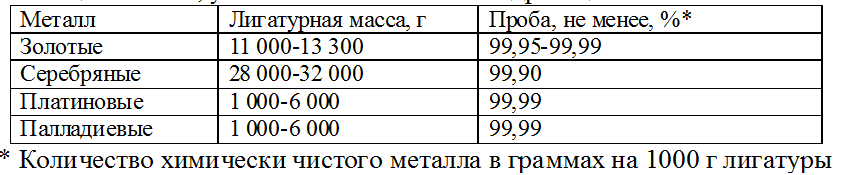
\includegraphics[scale=0.5]{img/gost.png}
\end{table}
\end{frame}

\begin{frame}[ allowframebreaks]{Оценка драгоценных камней}
Методика оценки камней массой более 1 карата:
\begin{align}
\text{С} = 0,5 * \text{Р} * (\text{Р} + 2) * \text{Ц},
\end{align}
где	С   – общая стоимость алмаза, дол. (или в другой валюте);

Р   – масса кристалла алмаза, караты; 

Ц  – цена за 1 карат алмаза, дол. (или в другой валюте).

\pagebreak
Цена за 1 карат определяется по специальным каталогам гомологических служб, составленных на основе прецедентов или особо авторитетными специалистами-экспертами. 

Эта цена зависит от общей массы камня, правильности форм кристалла, чистоты, цвета и его оттенков, отсутствия или наличия дефектов в виде трещин, сколов и т.п. 

При этом, чем крупнее кристалл, тем дороже стоимость 1 карата.

\end{frame}

\subsection{Рынок драгметаллов}
\begin{frame}{Рынок драг. металлов}
\begin{table}	
	\centering
	\caption{Мировое предложение и спрос на золото. }
	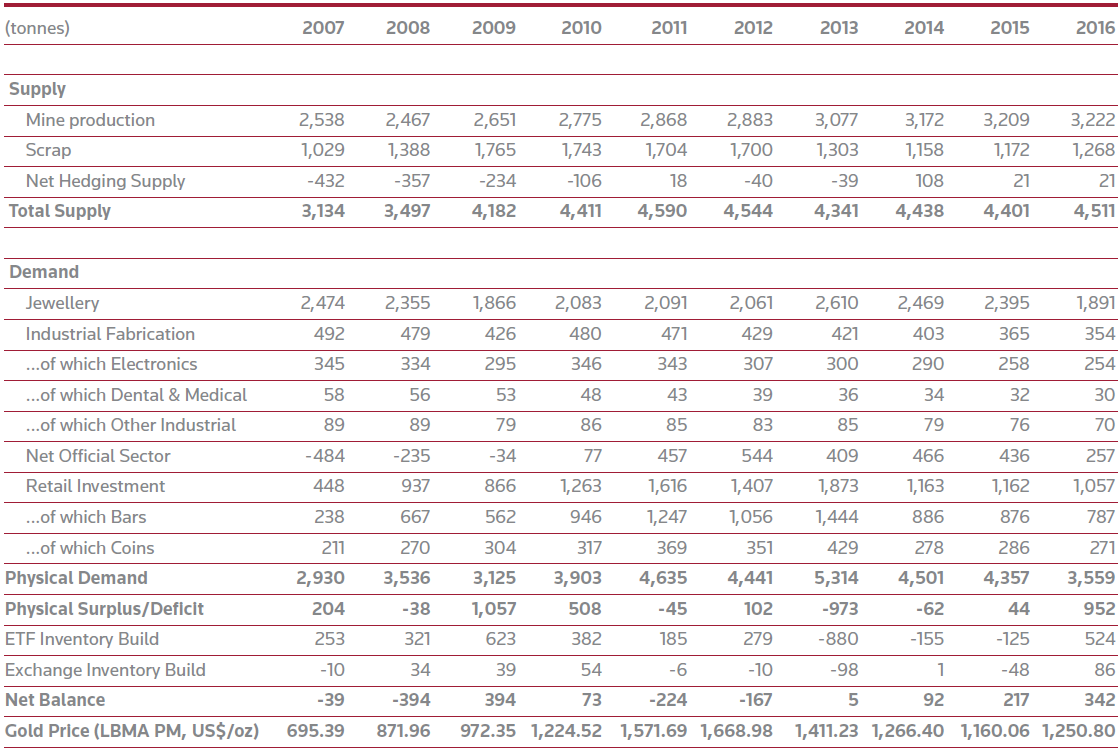
\includegraphics[scale=0.3]{img/world_gold_supply_and_demand.png}
\label{fig:world_gold_supply_and_demand}
\end{table}
Источник: \href{http://financial-risk-solutions.thomsonreuters.info/GFMS}{Gold Fields Mineral Services (GFMS) Gold Survey, Thomson Reuters. 2017.}
\end{frame}

\begin{frame}{}
\begin{table}
	\centering
	\caption{10 стран мира с крупнейшей добычей золота.}
	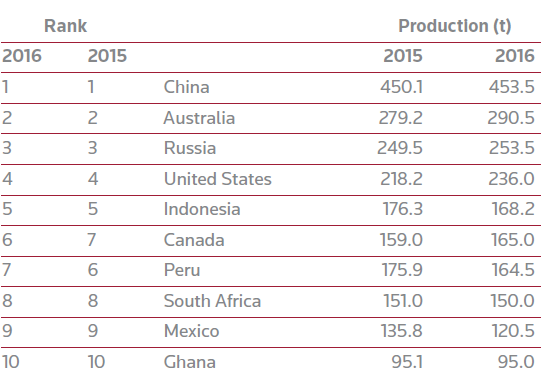
\includegraphics[scale=0.5]{img/top_10_gold_mining_countries.png}
\label{tbl:top_10_gold_mining_countries}
\end{table}
Источник: \href{http://financial-risk-solutions.thomsonreuters.info/GFMS}{Gold Fields Mineral Services (GFMS) Gold Survey, Thomson Reuters. 2017.}
\end{frame}

\begin{frame}[shrink=20]
\begin{figure}	
	\centering
	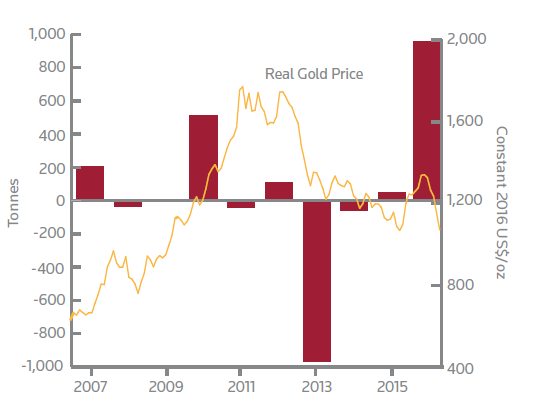
\includegraphics[scale=0.7]{img/gold_fisical_surplus_deficit.png}
	\caption{Физические избыток и дефицит золота в мире. \\Source: \href{http://financial-risk-solutions.thomsonreuters.info/GFMS}{Gold Fields Mineral Services (GFMS) Gold Survey, Thomson Reuters. 2017.}}\label{fig:gold_fisical_surplus_deficit}
\end{figure}
\end{frame}

\begin{frame}[shrink=20]
\begin{figure}	
	\centering
	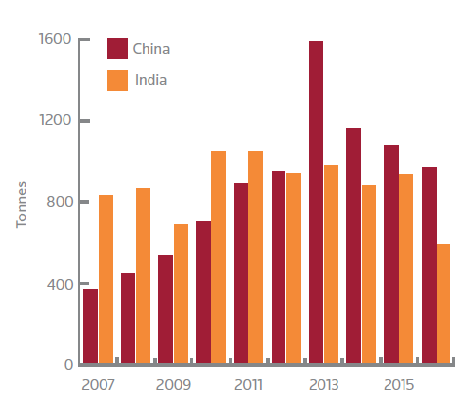
\includegraphics[scale=0.7]{img/china_india_gold_demand.png}
	\caption{Спрос на золото со стороны Индии и Китая. \\Source: \href{http://financial-risk-solutions.thomsonreuters.info/GFMS}{Gold Fields Mineral Services (GFMS) Gold Survey, Thomson Reuters. 2017.}}
	\label{fig:china_india_gold_demand}
\end{figure}
\end{frame}

\begin{frame}[shrink=20]
\begin{figure}	
	\centering
	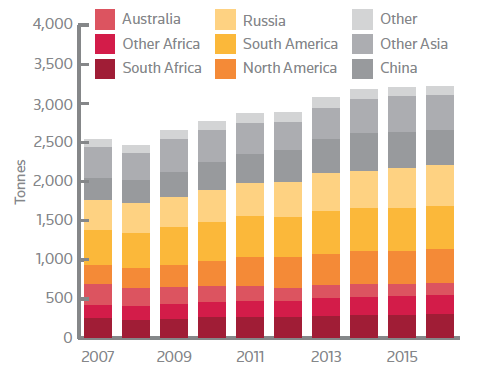
\includegraphics[scale=0.8]{img/global_gold_production.png}
	\caption{Объемы мирового производства золота. \\Source: \href{http://financial-risk-solutions.thomsonreuters.info/GFMS}{Gold Fields Mineral Services (GFMS) Gold Survey, Thomson Reuters. 2017.}}
	\label{fig:global_gold_production}
\end{figure}
\end{frame}

\begin{frame}[shrink=20]
\begin{figure}	
	\centering
	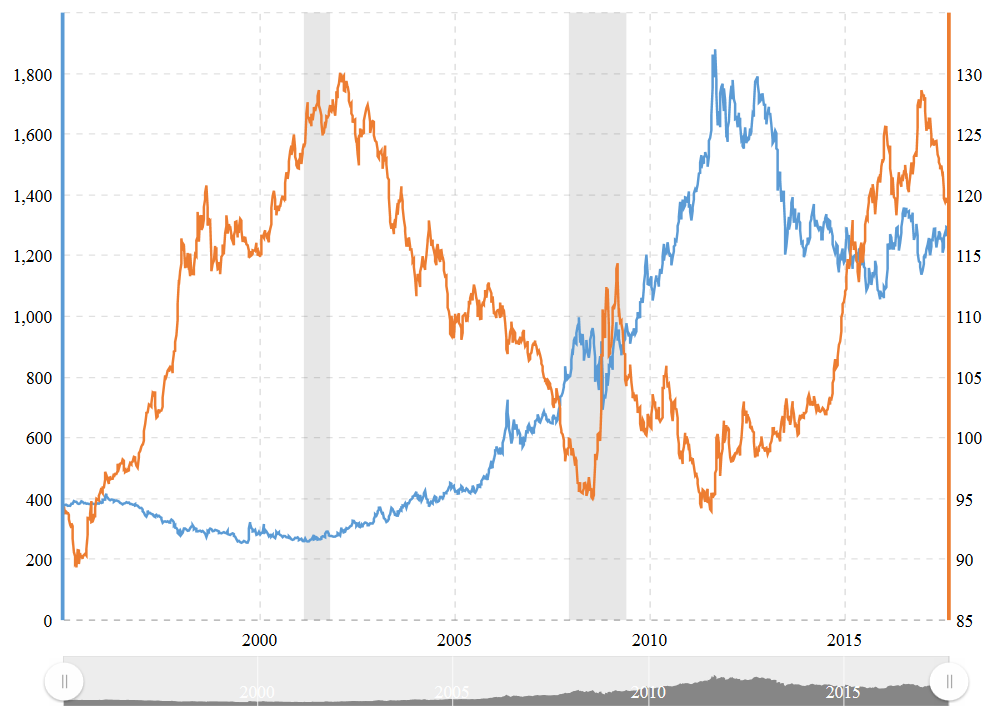
\includegraphics[scale=0.4]{img/gold_price_dollar_index.png}
	\caption{Динамика цены на золото в сравнении со средневзвешенным по объемам торговли индексом доллара. \\Source: \href{http://financial-risk-solutions.thomsonreuters.info/GFMS}{Gold Fields Mineral Services (GFMS) Gold Survey, Thomson Reuters. 2017.}}
	\label{fig:gold_price_dollar_index}
\end{figure}
\end{frame}

\begin{frame}{}
\begin{table}	
	\centering
	\caption{Себестоимость производства золота.}
	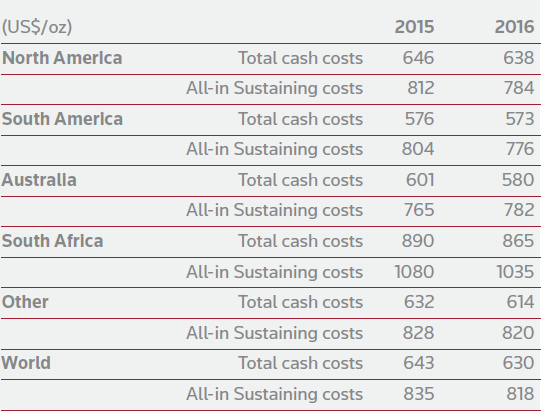
\includegraphics[scale=0.5]{img/gold_costs.png}
	\label{fig:gold_costs}
\end{table}
Источник: \href{http://financial-risk-solutions.thomsonreuters.info/GFMS}{Gold Fields Mineral Services (GFMS) Gold Survey, Thomson Reuters. 2017.}
\end{frame}

\begin{frame}{}
\begin{figure}	
	\centering
	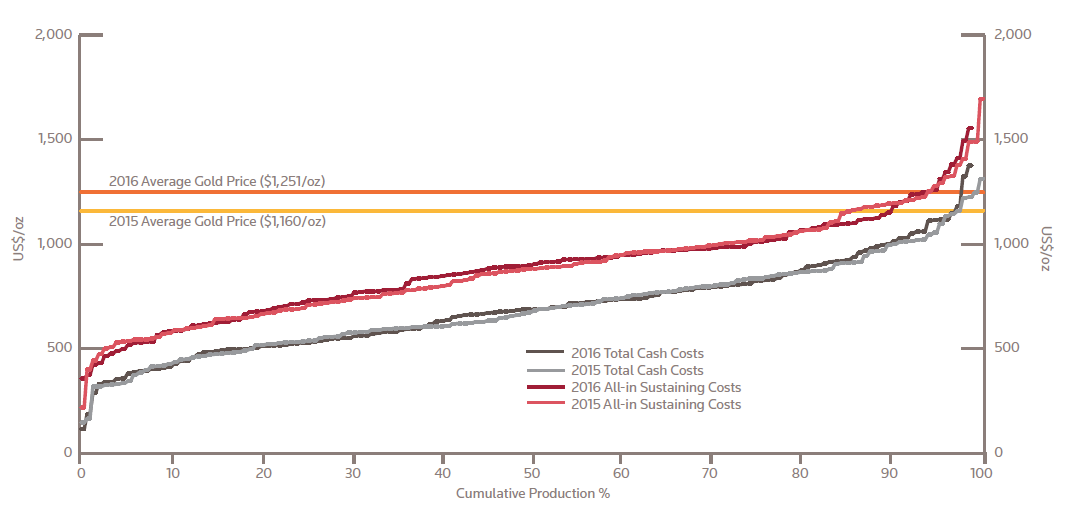
\includegraphics[scale=0.4]{img/gold_cost_curves.png}
	\caption{Кривые себестоимости производства золота. \\Source: \href{http://financial-risk-solutions.thomsonreuters.info/GFMS}{Gold Fields Mineral Services (GFMS) Gold Survey, Thomson Reuters. 2017.}}
	\label{fig:gold_cost_curves}
\end{figure}
\end{frame}

\begin{frame}[shrink=20]{}
\begin{figure}	
	\centering
	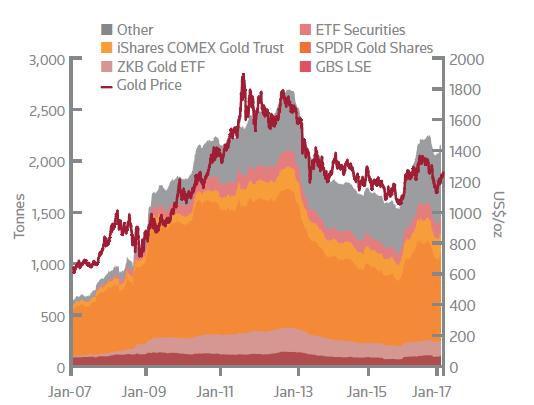
\includegraphics[scale=0.7]{img/gold_etfs.png}
	\caption{Объемы вложений в золото со стороны биржевых паевых фондов. \\Source: \href{http://financial-risk-solutions.thomsonreuters.info/GFMS}{Gold Fields Mineral Services (GFMS) Gold Survey, Thomson Reuters. 2017.}}
	\label{fig:gold_etfs}
\end{figure}
\end{frame}

\begin{frame}[shrink=25]
\begin{table}[htbp]
  \centering
  \caption{Страны с крупнейшими запасами золота на июнь 2017}
    \begin{tabular}{clrr}
    \toprule
    Ранг  & Страна & тонн  & доля в резервах \\
    \midrule
    1     & United States & 8133,5 & 74,5\% \\
    2     & Germany & 3374,1 & 69,0\% \\
    3     & IMF   & 2814,0 & - \\
    4     & Italy & 2451,8 & 66,9\% \\
    5     & France & 2435,9 & 63,6\% \\
    6     & China & 1842,6 & 2,3\% \\
    7     & Russia & 1715,8 & 16,6\% \\
    8     & Switzerland & 1040,0 & 5,4\% \\
    \bottomrule
    \multicolumn{4}{l}{Источник: World Gold Council, 2017.}\\
    \multicolumn{4}{l}{\url{http://www.gold.org/}}
    \end{tabular}%
  \label{tab:addlabel}%
\end{table}%
\end{frame}

\begin{frame}
\begin{figure}	
	\centering
	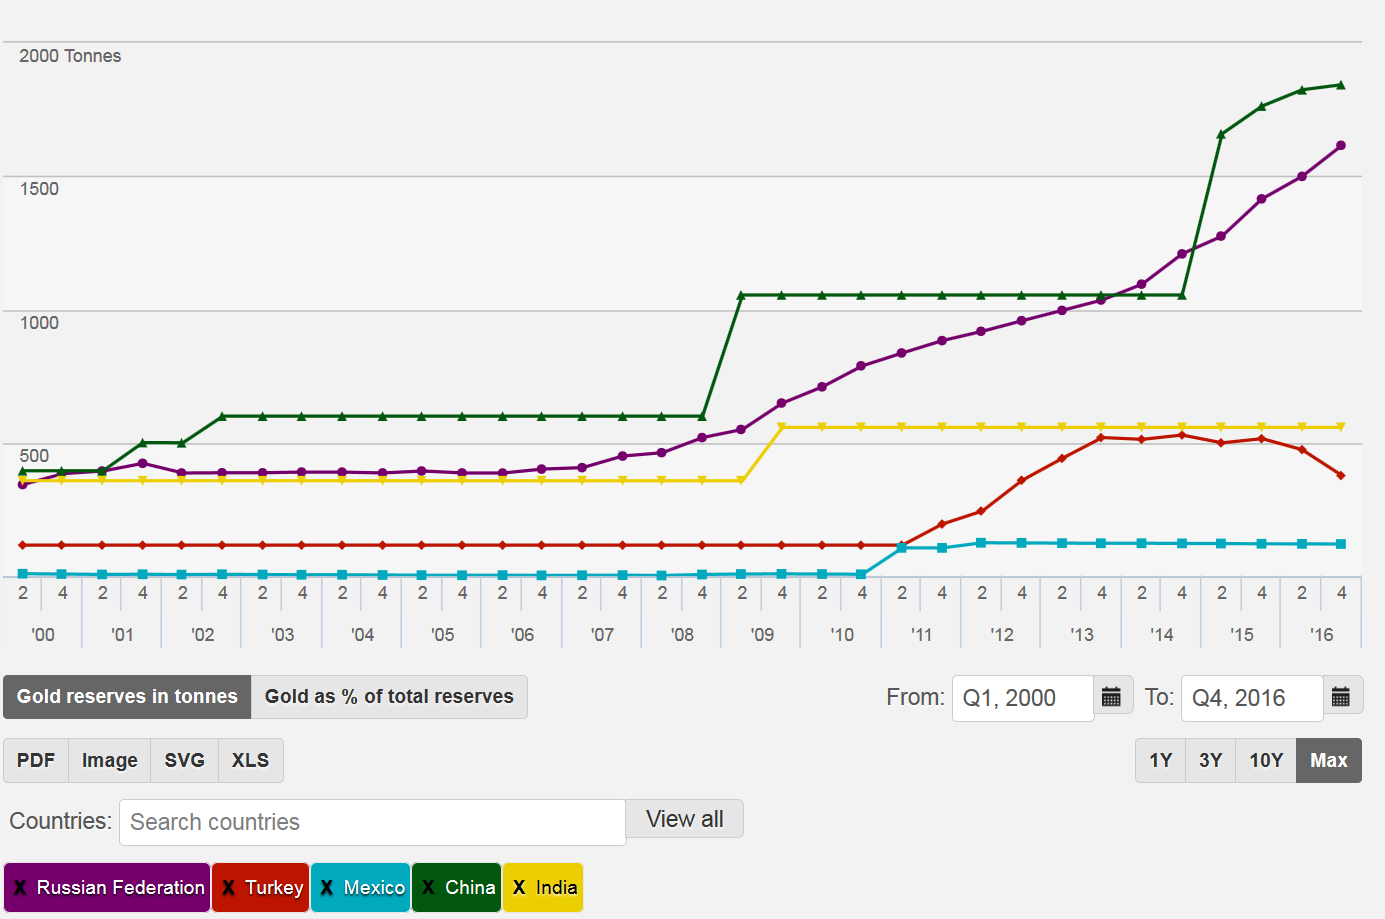
\includegraphics[scale=0.25]{img/official_reserves.png}
	\caption{Динамика официальных резервов золота у стран-крупнейших держателей. \\Источник: World Gold Council, 2017.\\ \url{http://www.gold.org/}}
	\label{fig:official_reserves}
\end{figure}
\end{frame}

\begin{frame}[shrink=20]
\begin{table}[htbp]
  \centering
  \caption{Доходность драгоценных металлов\\ на 31 июля 2017}
	\begin{tabularx}{\linewidth}[b]{@{}>{\raggedright\arraybackslash}Xrrrr@{}}
		\toprule
		        & Gold     & Silver   & Palladium & Platinum \\ \midrule
		1-month & 1,93\%   & -0,42\%  & 4,14\%    & 2,19\%   \\
		3-month & 0,09\%   & -3,73\%  & 7,35\%    & -0,51\%  \\
		YTD     & 10,62\%  & 4,36\%   & 31,59\%   & 4,52\%   \\
		1-year  & -5,55\%  & -16,37\% & 24,85\%   & -18,11\% \\
		3-year  & -1,38\%  & -18,99\% & 1,77\%    & -35,60\% \\
		5-year  & -21,85\% & -40,57\% & 50,57\%   & -33,56\% \\
		3y CAGR & -0,46\%  & -6,78\%  & 0,59\%    & -13,65\% \\
		5y CAGR & -4,81\%  & -9,88\%  & 8,53\%    & -7,85\%  \\ \bottomrule
	\end{tabularx}%
  \label{tab:addlabel}%

CAGR = compounded annual growth rate.

Source: Barclays Capital, Bloomberg, ICE Benchmark Administration Ltd, MSCI, World Gold Council, 2017. \url{http://www.gold.org/}
\end{table}%
\end{frame}

\begin{frame}[shrink=20]
\begin{table}[htbp]
  \centering
  \caption{Доходность индексов сырьевых товаров\\ на 31 июля 2017}
	\begin{tabularx}{\linewidth}[b]{@{}>{\raggedright\arraybackslash}Xrrrr@{}}
		\toprule
		        & Aluminum & Copper   & Lead    & Nickel   \\ \midrule
		1-month & 0,16\%   & 7,22\%   & 2,30\%  & 9,96\%   \\
		3-month & 0,34\%   & 11,05\%  & 2,30\%  & 8,10\%   \\
		YTD     & 14,23\%  & 16,07\%  & 10,78\% & 0,94\%   \\
		1-year  & 16,67\%  & 29,32\%  & 36,68\% & -3,90\%  \\
		3-year  & -3,52\%  & -10,48\% & 3,35\%  & -44,80\% \\
		5-year  & 1,54\%   & -15,75\% & 18,78\% & -35,61\% \\
		3y CAGR & -1,19\%  & -3,62\%  & 1,11\%  & -17,97\% \\
		5y CAGR & 0,31\%   & -3,37\%  & 3,50\%  & -8,43\%  \\ \bottomrule
	\end{tabularx}%
  \label{tab:addlabel}%

\raggedright
CAGR = compounded annual growth rate.

Source: Barclays Capital, Bloomberg, ICE Benchmark Administration Ltd, MSCI, World Gold Council, 2017. \url{http://www.gold.org/}
\end{table}%
\end{frame}

\begin{frame}[shrink=20]
\begin{table}[htbp]
  \centering
  \caption{Доходность индексов сырьевых товаров\\ на 31 июля 2017}
	\begin{tabularx}{\linewidth}[b]{@{}>{\raggedright\arraybackslash}Xrrrr@{}}
		\toprule
		        & Tin     & Zinc    & Brent    & S\&P Commodity \\ \midrule
		1-month & 2,71\%  & 5,39\%  & 11,50\%  & 3,10\%         \\
		3-month & 2,71\%  & 5,39\%  & 2,54\%   & 2,23\%         \\
		YTD     & -0,99\% & 10,31\% & -6,12\%  & -6,12\%        \\
		1-year  & 29,28\% & 45,63\% & 27,21\%  & 7,94\%         \\
		3-year  & -8,76\% & 16,75\% & -49,79\% & -52,95\%       \\
		5-year  & 14,88\% & 51,49\% & -50,76\% & -52,52\%       \\
		3y CAGR & -3,01\% & 5,30\%  & -20,52\% & -22,23\%       \\
		5y CAGR & 2,81\%  & 8,66\%  & -13,21\% & -13,84\%       \\ \bottomrule
	\end{tabularx}%
  \label{tab:addlabel}%

\raggedright
CAGR = compounded annual growth rate.

Source: Barclays Capital, Bloomberg, ICE Benchmark Administration Ltd, MSCI, World Gold Council, 2017. \url{http://www.gold.org/}
\end{table}%

\end{frame}

\begin{frame}[shrink=20]
\begin{table}[htbp]
  \centering
  \caption{Доходность индексов сырьевых товаров\\ на 31 июля 2017}
	\begin{tabularx}{\linewidth}[b]{@{}>{\raggedright\arraybackslash}Xrrrr@{}}
		\toprule
		        & Commodity & Energy   & Grains   & Livestock \\ \midrule
		1-month & 1,63\%    & 6,21\%   & -5,46\%  & -4,97\%   \\
		3-month & 0,90\%    & -2,90\%  & 0,09\%   & -3,33\%   \\
		YTD     & -3,11\%   & -17,19\% & 0,11\%   & 5,47\%    \\
		1-year  & 2,65\%    & -0,83\%  & 0,71\%   & 7,57\%    \\
		3-year  & -33,45\%  & -64,34\% & -24,45\% & -22,61\%  \\
		5-year  & -39,44\%  & -63,09\% & -50,47\% & -12,46\%  \\
		3y CAGR & -12,69\%  & -29,08\% & -8,92\%  & -8,19\%   \\
		5y CAGR & -9,54\%   & -18,07\% & -13,11\% & -2,63\%   \\ \bottomrule
	\end{tabularx}%
  \label{tab:addlabel}%

\raggedright
CAGR = compounded annual growth rate.

Source: Barclays Capital, Bloomberg, ICE Benchmark Administration Ltd, MSCI, World Gold Council, 2017. \url{http://www.gold.org/}
\end{table}%

\end{frame}


\subsection{Операции ЦБ РФ}
\begin{frame}[allowframebreaks]{Драгоценные металлы и драгоценные камни} {Операции Банка России}
\begin{itemize}
\item
лицензирование операций коммерческих банков с драгоценными металлами;
\item
контроль за деятельностью коммерческих банков в части проведения последними операций с драгоценными металлами;

\pagebreak
\item
приобретение для пополнения международных резервов РФ золота, серебра, платины и палладия на условиях предварительного авансирования недропользователей – производителей драгоценных металлов или обслуживающих их коммерческих банков;
\end{itemize}
\end{frame}

\begin{frame} {Драгоценные металлы и драгоценные камни} {Операции Банка России}
\begin{itemize}[<+->]
\item
приобретение уникальных экземпляров драгоценных камней;
\item
экспорт золота, серебра, платины и палладия. (Экспорт других металлов платиновой группы – осмия, иридия рутения, родия – осуществляется Гохраном РФ.)
\end{itemize}
\end{frame}

\subsection{Операции банков}
\begin{frame}{Драгоценные металлы и драгоценные камни}{Операции российских банков}
\begin{itemize}[<+->]

\item
сделки купли-продажи драгоценных металлов с Банком России (заключается Генеральное соглашение);

\item
операции купли-продажи драгоценных металлов между уполномоченными банками (на основе договоров);

\item
операции купли-продажи драгоценных металлов на международном рынке;

\item
сделки купли-продажи драгоценных металлов с недропользователями;

\item
операции купли-продажи драгоценных металлов с физическими лицами.
\end{itemize}
\end{frame}

\begin{frame}{Драгоценные металлы и драгоценные камни}{Операции российских банков}
\begin{itemize}[<+->]

\item
Операции по привлечению во вклады и размещению в кредит драгоценных металлов.

\item
Предоставление кредитов под залог драгоценных металлов и драгоценных камней.

\item
Операции по хранению и перевозке драгоценных металлов и драгоценных камней.

\item
Операции банков с монетами и медалями из драгоценных металлов. 
\end{itemize}
\end{frame}


\begin{frame}{Драгоценные металлы и драгоценные камни}{Операции российских банков}
\begin{itemize}[<+->]
\item
Экспортные операции с драгоценными металлами. 

\item
Операции с природными драгоценными камнями.

\item
сделки с использованием опционов, свопов, форвардов, фьючерсов и других финансовых инструментов базовым активом по которым являются драгоценные металлы.
\end{itemize}
\end{frame}

\begin{frame}[shrink=25]
\begin{table}[htbp]
  \centering
  \caption{Цены покупки и продажи\\ мерных слитков золота на 17.08.2017, руб.}
    \begin{tabular}{crrr}
    \toprule
   
	\multirow{2}[4]{*}{ Номинал, г} & \multicolumn{2}{c}{Покупка: качество} & 				\multirow{2}[4]{*}{Продажа} \\\cmidrule(lr){2-3}
          & Удвл  & Отл   &  \\
    \midrule
    1     & 2 305 & 2 325 & 3 325 \\
    5     & 11 525 & 11 565 & 15 564 \\
    10    & 23 050 & 23 120 & 30 892 \\
    20    & 46 100 & 46 200 & 61 431 \\
    50    & 115 250 & 115 370 & 152 692 \\
    100   & 230 500 & 230 650 & 304 322 \\
    250   & 576 250 & 576 450 & 759 094 \\
    500   & 1 152 500 & 1 152 870 & 1 517 126 \\
    1000  & 2 305 000 & 2 305 600 & 3 032 954 \\
    \bottomrule
    \multicolumn{4}{l}{Источник:\href{http://www.sberbank.ru/ru/person/contributions/values/metall}{Сбербанк России}.}
    \end{tabular}%
  \label{tab:gold_bar_prices}%
\end{table}%

\end{frame}

\begin{frame}[shrink=25]
\begin{table}[htbp]
  \centering
  \caption{Цены покупки и продажи\\ мерных слитков серебра на 17.08.2017, руб.}
    \begin{tabular}{crrr}
    \toprule
   
	\multirow{2}[4]{*}{ Номинал, г} & \multicolumn{2}{c}{Покупка: качество} & 				\multirow{2}[4]{*}{Продажа} \\\cmidrule(lr){2-3}
          & Удвл  & Отл   &  \\
    \midrule
	50    & 1 533 & 1 563 & 2 427 \\
    100   & 3 066 & 3 136 & 4 735 \\
    250   & 7 665 & 7 815 & 11 071 \\
    500   & 15 330 & 15 580 & 21 494 \\
    1000  & 30 660 & 31 160 & 42 515 \\
    \bottomrule
    \multicolumn{4}{l}{Источник:\href{http://www.sberbank.ru/ru/person/contributions/values/metall}{Сбербанк России}.}
    \end{tabular}%
  \label{tab:silver_bar_prices}%
\end{table}%

\end{frame}
\begin{frame}
\begin{table}[htbp]
  \centering
  \caption{Цены покупки и продажи\\ мерных слитков платины на 17.08.2017, руб.}
    \begin{tabular}{crrr}
    \toprule
   
	\multirow{2}[4]{*}{ Номинал, г} & \multicolumn{2}{c}{Покупка: качество} & 				\multirow{2}[4]{*}{Продажа} \\\cmidrule(lr){2-3}
          & Удвл  & Отл   &  \\
    \midrule
    5     & 8 740 & 8 940 & 12 425 \\
    10    & 17 480 & 17 755 & 24 202 \\
    20    & 34 960 & 35 360 & 47 578 \\
    50    & 87 400 & 87 875 & 116 879 \\
    100   & 174 800 & 175 550 & 232 460 \\
    \bottomrule
    \multicolumn{4}{l}{Источник:\href{http://www.sberbank.ru/ru/person/contributions/values/metall}{Сбербанк России}.}
    \end{tabular}%
  \label{tab:platinum_bar_prices}%
\end{table}%

\end{frame}

\begin{frame}
\begin{table}[htbp]
  \centering
  \caption{Цены покупки и продажи\\ мерных слитков палладия на 17.08.2017, руб.}
    \begin{tabular}{crrr}
    \toprule
   
	\multirow{2}[4]{*}{ Номинал, г} & \multicolumn{2}{c}{Покупка: качество} & 				\multirow{2}[4]{*}{Продажа} \\\cmidrule(lr){2-3}
          & Удвл  & Отл   &  \\
    \midrule
    5     & -------- & -------- & 12136 \\
    10    & -------- & -------- & 23447 \\
    20    & -------- & -------- & 45241 \\
    50    & -------- & -------- & 111215 \\
    100   & -------- & -------- & 219657 \\
    \bottomrule
    \multicolumn{4}{l}{Источник:\href{http://www.sberbank.ru/ru/person/contributions/values/metall}{Сбербанк России}.}
    \end{tabular}%
  \label{tab:palladium_bar_prices}%
\end{table}%

\end{frame}


\subsection{Банковские риски}
\begin{frame} {Банковские риски}{по операциям с драгоценными металлами и драгоценными камнями}
\begin{itemize}[<+->]
\item
ценовой риск, связанный с возможностью возникновения потерь от неблагоприятного непредвиденного изменения цен на драгоценные металлы (драгоценные камни);

\item 
риск потери ликвидности, связанный с возможностью появления убытков при управлении активами и пассивами коммерческого банка в драгоценных металлах (драгоценных камнях), не сбалансированными по срокам и суммам;
\end{itemize}
\end{frame}

\begin{frame} {Банковские риски}{по операциям с драгоценными металлами и драгоценными камнями}
\begin{itemize}[<+->]
\item
правовой риск, связанный с возможностью возникновения убытков в результате принятия новых нормативных документов, касающихся деятельности банков, или изменения действующих;

\item
риски, связанные с операциями по авансированию закупок драгоценных металлов у недропользователей, а также кредитованию предприятий золотодобывающей промышленности и предприятий по добыче других драгоценных металлов и драгоценных камней.
\end{itemize}
\end{frame}



\subsection{Контрольные вопросы}
\begin{frame}[ allowframebreaks ]{Контрольные вопросы}
1. Понятие, виды, стандарты выпуска драгоценных металлов. Проба металла. Лигатура.

2. Понятия добычи, производства, аффинажа драгоценных металлов.

3. Понятие, виды, удиницы измерений веса драгоценных камней. 

4. Методика оценки драгоценных камней весом более 1 карата.

\pagebreak
5. Характеристика мирового рынка драгоценных металлов.

6. Операции Банка России с драгоценными металлами и драгоценными камнями.

7. Операции российских банков с драгоценными металлами и драгоценными камнями.

8. Банковские риски по операциям с драгоценными металлами и драгоценными камнями.
\end{frame}

\setbeamercovered{transparent}
\end{document}
